Вторая формула грина:
\[ 
			\iint\limits_S \left(u \der{v}{n}{} - v \der{u}{n}{}\right) d\sigma = \iiint\limits_{W} \left(u \Delta v - v \Delta u \right) d \tau
\]
Рассмотрим трёхмерную задачу Дирихле. 
\[
	\Delta u = 0
\]
\[
	u\big|_S = f
\]
\begin{wrapfigure}{r}{0.3\textwidth}
	\centering
	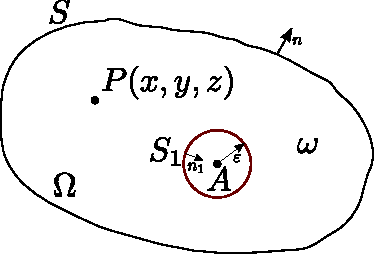
\includegraphics[width = 0.3\textwidth]{figGreenThreeDim.pdf}
\end{wrapfigure}
Применим вторую формулу Грина к этой задаче.\\

В области $\Omega$ возьмём $(\cdot)A(x_0, y_0, z_0)$ и произвольную $(\cdot)P(x, y, z)$.
\[
	r_{AP} = \sqrt{(x - x_0)^2 + (y - y_0)^2 + (z - z_0)^2}\quad \text{радиус между $A$ и $P$}
\]
Покажем, что $w = \frac{1}{r_{AP}}$ удовлетворяет уравнению Лапласа $\Delta u = 0$:
\[
	\Delta u = \derp{u}{x}{2} + \derp{u}{y}{2} + \derp{u}{z}{2} = 0
\]
Найдём вторые производные и подставим в уравнение:
\[
	\derp{w}{x}{} = - \frac{1}{r_{AP}^2} \derp{r_{AP}}{x}{} = - \frac{1}{r_{AP}^2} \frac{ (x - x_0)}{  \sqrt{(x - x_0)^2 + (y - y_0)^2 + (z - z_0)^2}} = - \frac{(x - x_0)}{r_{AP}^3}
\]
\begin{align*}
	\derp{w}{x}{2} &= - \frac{1}{r_{AP}^3} + \frac{3 (x - x_0)}{r_{AP}^5}\\
	\derp{w}{y}{2} &= - \frac{1}{r_{AP}^3} + \frac{3 (y - y_0)}{r_{AP}^5}\\
	\derp{w}{z}{2} &= - \frac{1}{r_{AP}^3} + \frac{3 (z - z_0)}{r_{AP}^5}
\end{align*}
\[
	\Delta u - \frac{3}{r_{AP}^3} + \frac{3 [(x - x_0)^2 + (y - y_0)^2 + (z - z_0)^2]}{r_{AP}^5} \equiv 0
\]
Действительно $w = \frac{1}{r_{AP}}$ удовлетворяет уравнению Лапласа, то есть является гармонической.\\[5pt]
Должное решение в $(\cdot)A$ имеет особенность. Окружаем $(\cdot)A$ сферой малого радиуса $\varepsilon$. $w$ --- область между двумя сферами. Тогда формула Грина принимает вид:
\[
	\iint\limits_S \left(u \der{v}{n}{} - v \der{u}{n}{}\right) dS + \iint\limits_{S_1} \left(u \der{v}{n_1}{} - v \der{u}{n_1}{}\right) dS_1 = \iiint\limits_\omega \left(u \Delta v - v \Delta u \right) d \omega
\]

Функция $w$  в области $\omega$ не имеет особенностей. Во всей области строим решение $w_1$, которое имеет особенность. 

Потребуем, чтобы $\Delta w_1 = 0; w_1 \big|_S = W\big|_S$. Построим функцию Грина:
\[
	G(x, y, z, x_0, y_0, z_0) = w_1 - w
\]
Тогда на границе: 
\[
	G\big|_S = 0
\]
Предположим, что в формуле Грина $v = G$.
\[
	\iint\limits_S \left(u \der{v}{n}{} - v \underbrace{\der{u}{n}{}}_0\right) dS + \iint\limits_{S_1} \left(u \der{v}{n_1}{} - v \der{u}{n_1}{}\right) dS_1 = 0
\]
Получаем 
\[
	\iint\limits_S u \derp{G}{n}{}\, dS + \iint\limits_{S_1} \left(u \der{G}{n_1}{} - G \der{u}{n_1}{}\right) dS_1 = 0
\]

\begin{wrapfigure}{l}{0.3\textwidth}
	\centering
	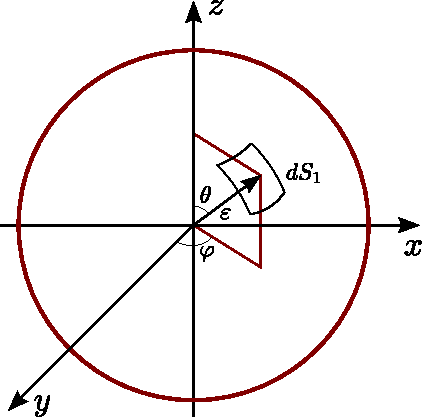
\includegraphics[width = 0.3\textwidth]{figGreenIllust.pdf}
\end{wrapfigure}
Перейдём к сферической системе координат во втором интеграле:
\begin{align*}
	&dS_1 = \varepsilon^2 \sin \theta\, d \theta d \varphi\\
	&0 \leqslant \theta \leqslant \pi; \quad 0 \leqslant \varphi \leqslant 2\pi\\
	&\derp{}{n_1}{} = - \derp{}{r}{}
\end{align*}

\[
	 \iint\limits_{S_1} \left(u \der{G}{n_1}{} - G \der{u}{n_1}{}\right) dS_1 = \int\limits_0^{2 \pi}\, d\varphi \int\limits_0^{\pi} \left(- u \der{G}{r}{} + G \der{u}{r}{} \right) \varepsilon \sin \theta\, d\theta
\]
\[
	G = w_1 - \frac{1}{r_{AP}}
\]
\begin{multline*}
	\iint\limits_{S_1} \left(u \derp{G}{n_1}{} - G \derp{u}{n_1}{} \right)\, dS = \iint\limits_{S_1} \Big(- u \derp{}{r}{} \Big(w_1 - \frac{1}{\underbrace{r_{AP}}_r} \Big) + \Big(w_1 - \frac{1}{\underbrace{r_{AP}}_r} \Big) \derp{u}{r}{} \Big)\, dS =\\
	= \iint\limits_{S_1} \left(- u \derp{w_1}{r}{} - \frac{1}{r^2} u + w_1 \derp{u}{r}{} - \frac{1}{r} \derp{u}{r}{}\right)\, dS = \\
	= \int\limits_0^{2 \pi}d \varphi \int\limits_0^\pi d \theta \left\{ - u \derp{w_1}{r}{} - \frac{1}{\varepsilon^2} u + w_1 \derp{u}{r}{} - \frac{1}{\varepsilon} \derp{u}{r}{} \right\} \varepsilon^2 \sin \theta
\end{multline*}

Будем устремлять радиус $\varepsilon$ к $0$:
\[
	\lim\limits_{\varepsilon \to 0} \iint\limits_{S_1} \left(u \derp{G}{n_1}{} - G \derp{u}{n_1}{} \right)\, dS = \lim\limits_{\varepsilon \to 0} \varepsilon^2 \int\limits_0^{2 \pi} d\varphi \int\limits_0^{2 \pi} d \theta \sin \theta \left\{ - u \derp{w_1}{r}{} - \frac{1}{\varepsilon^2} u + w_1 \derp{u}{r}{} - \frac{1}{\varepsilon} \derp{u}{r}{} \right\}
\]
\[
	\varepsilon^2 u \derp{w}{r}{} \to 0 \big|_{\varepsilon \to 0}
\]
\[
	\varepsilon^2 w_1 \derp{u}{r}{} \to 0; \quad \varepsilon \derp{u}{r}{} \to 0
\]
Получаем 
\[
	- \int\limits_0^{2 \pi} d \varphi \int\limits_0^\pi d\theta \sin \theta u - u(x_0, y_0, z_0) \int\limits_0^{2 \pi} d \varphi \int\limits_0^\pi \sin \theta = - 4 \pi u (x_0, y_0, z_0)
\]
Подставляем в формулу Грина:
\[
	\iint\limits_S u \derp{G}{n}{}\, dS - 4 \pi u (x_0, y_0, z_0) = 0
\]
\[
	u (x_0, y_0, z_0) = \frac{1}{4 \pi} \iint\limits_S f \derp{G}{n}{}\, dS
\]


